\documentclass[10pt,conference]{IEEEtran}
\IEEEoverridecommandlockouts

\usepackage{amsmath,amssymb,amsfonts}
\usepackage{booktabs}
\usepackage{graphicx}
\usepackage{textcomp}
\usepackage{xcolor}
\usepackage{algorithm}
\usepackage{algpseudocode}
\usepackage{listings}
\usepackage{cite}
\usepackage{url}
\usepackage{microtype}

\graphicspath{{figures/}}

% Track Changes / Highlighting for IEEE ICCIT 2026 Reviewers
\definecolor{revcolor}{RGB}{0, 40, 160}
\newenvironment{revised}{\color{revcolor}}{}
\newcommand{\rev}[1]{\textcolor{revcolor}{#1}}


% Tightly balance floats and text for strict 6-page ceiling
\setlength{\textfloatsep}{3pt plus 1pt minus 1pt}
\setlength{\floatsep}{3pt plus 1pt minus 1pt}
\setlength{\intextsep}{3pt plus 1pt minus 1pt}
\setlength{\dbltextfloatsep}{3pt plus 1pt minus 1pt}
\setlength{\dblfloatsep}{3pt plus 1pt minus 1pt}
\def\IEEEbibitemsep{0pt plus .05pt}

\lstdefinestyle{dartstyle}{
    basicstyle=\ttfamily\tiny,
    keywordstyle=\bfseries\color{blue!70!black},
    stringstyle=\color{green!50!black},
    commentstyle=\itshape\color{gray},
    numbers=left,
    numberstyle=\tiny\color{gray},
    stepnumber=1,
    numbersep=2pt,
    backgroundcolor=\color{gray!8},
    frame=single,
    rulecolor=\color{gray!30},
    tabsize=2,
    breaklines=true,
    breakatwhitespace=false,
    showspaces=false,
    showstringspaces=false
}

\newtheorem{definition}{Definition}
\newtheorem{theorem}{Theorem}
\newtheorem{lemma}{Lemma}

\begin{document}

\title{VisioCrypt: A TEE-Anchored Client-Side Searchable Encryption Scheme with Dynamic Volume-Hiding Padding for Mobile Cloud Storage}

\author{\IEEEauthorblockN{Anonymous Author(s) \quad {\normalsize\color{revcolor}[REVISION HIGHLIGHTED VERSION]}}
\IEEEauthorblockA{Paper ID: 2015}}

\maketitle
\thispagestyle{empty}
\pagestyle{empty}

\begin{abstract}
Mobile cloud storage allows users to synchronize sensitive documents across personal devices, yet delegating storage to untrusted cloud providers risks catastrophic data exposure during server breaches. While Searchable Symmetric Encryption (SSE) enables keyword lookups over encrypted records without full-corpus downloading, conventional schemes leak matching candidate volumes and access patterns. Passive cloud adversaries exploit this volume leakage to reconstruct plaintexts. Furthermore, mobile platforms suffer from severe memory hygiene vulnerabilities, where runtime garbage collection leaves transient cryptographic keys exposed in volatile memory for extended intervals.

In this paper, we propose \textbf{VisioCrypt}, a client-side dynamic searchable encryption framework co-designed for resource-constrained mobile architectures. VisioCrypt introduces a multi-tiered geometric volume-hiding padding policy $\Phi(R)$ that rounds matching candidate lists to discrete power-of-two boundaries ($n \in [1, 4096]$) with multi-bucket chunking, strictly bounding volume leakage to $\lceil \log_2 |R(w)| \rceil$ with an average storage expansion of only $1.42\times$. Master root keys are anchored in hardware-backed mobile enclaves (ARM TrustZone / Android KeyMint) with biometric gating, while operational keys are derived via domain-separated HKDF-SHA256 protocols. Transient keys in memory-isolated worker threads are actively wiped using best-effort buffer zeroization. Deletions are processed via an in-memory Bloom filter mathematically proven to serve as a negative lookup accelerator, preventing false document exclusions. We provide formal simulation-based security definitions ($\mathcal{L}_{\text{dyn-VH}}\text{-IND-CKA2}$) and a complete 5-game hopping proof. Empirical evaluation across four physical Android hardware tiers confirms sub-millisecond search latencies ($0.23$--$1.48$~ms), file streaming throughput up to $310$~MB/s, and query decorrelation that reduces adversary profiling accuracy to random guessing ($50.6\%$).
\end{abstract}

\begin{IEEEkeywords}
Searchable symmetric encryption, dynamic volume-hiding padding, ARM TrustZone, mobile security, leakage-abuse attacks.
\end{IEEEkeywords}

\section{Introduction}
Centralized cloud storage services (e.g., Google Drive, Dropbox) provide scalable document availability for mobile users. However, storing plaintext files in public cloud infrastructure forces users to surrender physical custody of their sensitive personal, financial, and medical data. Breaches resulting from server misconfigurations, compromised hypervisors, or rogue administrators routinely compromise user confidentiality \cite{islam2012,cash2015leakage}. To guarantee data sovereignty and adhere to stringent privacy frameworks (e.g., GDPR, HIPAA), client-side encryption prior to cloud transmission is imperative.

Nonetheless, naive end-to-end encryption transforms structured documents into opaque, unstructured ciphertexts. Under this paradigm, executing a search query for a specific document requires the mobile client to download, buffer, and decrypt the entire encrypted repository locally. On resource-constrained mobile devices operating over metered cellular connections, this imposes prohibitive bandwidth consumption, severe latency, and rapid battery exhaustion.

Searchable Symmetric Encryption (SSE), pioneered by Song, Wagner, and Perrig (SWP00) \cite{song2000} and formalized with optimal inverted indexes by Curtmola et al. (CGKO06) \cite{curtmola2006}, resolves this operational dilemma. In SSE, an untrusted cloud server traverses an encrypted index to locate matching records using cryptographic search tokens (trapdoors) generated by the client, without learning underlying plaintext contents. Kamara et al. \cite{kamara2012} extended SSE to dynamic collections supporting document insertions and deletions.

Despite theoretical progress, deploying dynamic SSE on real-world mobile platforms exposes three critical vulnerabilities:
\begin{enumerate}
    \item \textbf{Volume and Frequency Leakage:} Standard SSE constructions reveal the exact number of matching ciphertexts ($|R(w)|$) for any queried keyword $w$. State-of-the-art leakage-abuse attacks (e.g., Kellaris et al. \cite{kellaris2016}, Gui et al. \cite{gui2019volume}) demonstrate that an adversary observing query frequencies and result set sizes can reconstruct the underlying document database and decrypt user queries in polynomial time. Existing volume-hiding defenses, such as SEAL \cite{demertzis2020seal} and DVH \cite{patel2023dvh}, rely on complex oblivious RAM structures or server-side binning that induce high bandwidth overhead ($3\times$--$10\times$) and computational roundtrips impractical for mobile radios.
    \item \textbf{Mobile Runtime Memory Insecurity:} Academic SSE literature predominantly models client devices as secure, ideal Turing machines. In reality, mobile platforms execute managed runtimes (e.g., Android ART, Dart VM) governed by non-deterministic garbage collection (GC). Discarded cryptographic key objects persist unzeroized in heap memory for minutes, leaving them vulnerable to unprivileged cold-boot attacks, root exploits, and memory-dump side channels \cite{kocher1996,rustee2020}.
    \item \textbf{Temporal Profiling and Traffic Correlation:} An eavesdropper monitoring encrypted network channels can correlate packet dispatch timing with user typing dynamics or specific application states \cite{swat2024}. Naive randomized query delays fail against statistical averaging over repeated sessions.
\end{enumerate}

To overcome these foundational limitations, we present \textbf{VisioCrypt}, a secure, TEE-anchored client-side dynamic searchable encryption system designed specifically for mobile cloud storage. VisioCrypt balances formal cryptographic leakage mitigation with practical mobile efficiency. Specifically, our contributions are:
\begin{itemize}
    \item \textbf{Multi-Tier Dynamic Volume-Hiding SSE ($\text{DVH-SSE}$):} We formulate a client-centric geometric padding policy $\Phi(R)$ that rounds matching candidate lists into power-of-two buckets ($n \in [1, 4096]$) with multi-bucket chunking for large result sets. This restricts server-visible volume leakage strictly to $\lceil \log_2 |R(w)| \rceil$, slashing volumetric attack surfaces while bounding storage expansion to $1.42\times$.
    \item \textbf{Hardware-Anchored Key Lifecycle \& Memory Hygiene:} We root VisioCrypt's master secret in client-side hardware security modules (ARM TrustZone / Android KeyMint / StrongBox) gated by biometric authorization (\texttt{BiometricPrompt}). Operational keys are derived through RFC 5869 HKDF-SHA256 domain separation. Cryptographic executions run inside isolated Dart worker threads with active buffer zeroization, mitigating heap persistence risks.
    \item \textbf{Provably Correct Negative-Lookup Deletion Filter:} We integrate an in-memory Bloom filter for client-side deletion acceleration. We mathematically prove that false positives incur bounded verification overhead rather than false document exclusions, ensuring zero correctness degradation.
    \item \textbf{Traffic Decorrelation \& Formal Adaptive Security:} We introduce a \texttt{QueryDecorrelationPool} that batches queries into discrete epochs with injected dummy trapdoors, reducing timing attack classification accuracy to random guessing ($50.6\%$). We prove that VisioCrypt achieves adaptive $\mathcal{L}_{\text{dyn-VH}}\text{-IND-CKA2}$ security via a 5-game hopping proof.
    \item \textbf{Multi-Tier Physical Mobile Evaluation:} We evaluate VisioCrypt across four physical Android hardware tiers (flagship Snapdragon 8 Gen 3 down to entry-level Helio G80). Results confirm sub-millisecond search resolution ($0.23$--$1.48$~ms), file streaming throughput up to $310$~MB/s, and negligible battery consumption.
\end{itemize}

\enlargethispage{2\baselineskip}

\begin{revised}
\section{Related Work and Foundations}
\subsection{Searchable Symmetric Encryption Foundations}
Song, Wagner, and Perrig (SWP00) \cite{song2000} introduced the first practical mechanism for searching encrypted data. The SWP00 scheme operates by encrypting individual words using a two-layered stream cipher and keyed pseudo-random function (PRF) construction ($C_i = W_i \oplus \langle L_i, R_i \rangle$). To search for a keyword, the client supplies a trapdoor enabling the server to evaluate whether $R_i = f_k(L_i)$ without decrypting the underlying word. While groundbreaking, SWP00 requires an $O(N)$ sequential scan over the entire document ciphertext space, incurring severe computation and battery drain on mobile devices. Furthermore, SWP00 lacked formal security definitions and inverted index structures.

Curtmola, Garay, Kamara, and Ostrovsky (CGKO06) \cite{curtmola2006} formalized modern SSE security, establishing rigorous simulation-based definitions (non-adaptive IND-CKA1 and adaptive IND-CKA2) and introducing inverted-index SSE constructions based on array lookups. By decoupling search time from total repository size, CGKO06 achieved optimal $O(|R(w)|)$ query complexity. However, the original CGKO06 construction is static; updating or deleting documents requires a complete, costly index rebuild.

\begin{table*}[t]
\centering
\caption{Qualitative Comparison of Searchable Symmetric Encryption (SSE) Schemes Across Cryptographic and Mobile Dimensions}
\label{tab:comparison}
\scriptsize
\setlength{\tabcolsep}{3.5pt}
\renewcommand{\arraystretch}{0.95}
\begin{tabular}{lcccccccc}
\toprule
\textbf{Scheme} & \textbf{Search Complexity} & \textbf{Update Complexity} & \textbf{Forward Privacy} & \textbf{Backward Privacy} & \textbf{Volume Hiding} & \textbf{Result-Size Leakage} & \textbf{TEE Dependency} & \textbf{Mobile Suitability} \\
\midrule
Song et al. (SWP00) \cite{song2000} & $O(N)$ & $O(1)$ & No & No & No & Exact $|R(w)|$ & None & Poor (High battery drain) \\
Curtmola et al. (CGKO06) \cite{curtmola2006} & $O(|R(w)|)$ & Static (No updates) & N/A & N/A & No & Exact $|R(w)|$ & None & Moderate (Static only) \\
Kamara et al. (KPR12) \cite{kamara2012} & $O(|R(w)|)$ & $O(d_w)$ & No & No & No & Exact $|R(w)|$ & None & Moderate \\
Cash et al. \cite{cash2013} & $O(|R(w)|)$ & Static / Append & No & No & No & Exact $|R(w)|$ & None & Good (Large scale) \\
Bost (Sophos) \cite{bost2016sophos} & $O(|R(w)|)$ & $O(1)$ & \textbf{Yes} & No & No & Exact $|R(w)|$ & None & Good \\
Bost et al. (Diana) \cite{bost2017diana} & $O(|R(w)|)$ & $O(1)$ & \textbf{Yes} & \textbf{Yes} (Type-II) & No & Exact $|R(w)|$ & None & Moderate \\
Demertzis et al. (SEAL) \cite{demertzis2020seal} & $O(|R(w)| + \log N)$ & $O(\log N)$ & \textbf{Yes} & \textbf{Yes} & \textbf{Yes} & Binned $B_i$ & None & Moderate (Bandwidth intensive) \\
Patel et al. (DVH) \cite{patel2023dvh} & $O(|R(w)|)$ & $O(\text{polylog } N)$ & \textbf{Yes} & \textbf{Yes} & \textbf{Yes} & Binned $O(\log N)$ & None & Low (Heavy client storage) \\
Liu et al. \cite{li2021trustzone} & $O(|R(w)|)$ & $O(1)$ & \textbf{Yes} & \textbf{Yes} & No & Exact $|R(w)|$ & Server TEE & Poor (Requires cloud enclave) \\
\midrule
\textbf{VisioCrypt (Ours)} & $\mathbf{O(1) + O(\Phi(|R|))}$ & $\mathbf{O(1)}$ & \textbf{Yes} & \textbf{Yes} (Type-II) & \textbf{Yes} & Padded $\lceil \log_2 |R(w)| \rceil$ & \textbf{Client-Side Only} & \textbf{High} (Sub-ms, zeroization) \\
\bottomrule
\end{tabular}
\end{table*}

\subsection{Dynamic SSE and Forward/Backward Privacy}
Kamara, Papamanthou, and Roeder (KPR12) \cite{kamara2012} extended SSE to dynamic settings using encrypted index pointers. However, naive dynamic SSE schemes leak correlations between past search queries and subsequent document updates. Zhang et al. \cite{zhang2016injection} demonstrated that an adversary injecting crafted documents can fully reconstruct queried keywords via file-injection attacks. To thwart injection attacks, Bost \cite{bost2016sophos} formalized \emph{Forward Privacy}: an update operation must not leak any association with previously searched keywords. Sophos achieved forward privacy through trapdoor permutations. Bost, Minaud, and Ohrimenko \cite{bost2017diana} subsequently formalized \emph{Backward Privacy} across three standard tiers (Type-I, Type-II, Type-III), ensuring that search queries do not expose document identifiers that have been deleted. Diana achieved backward privacy via puncturable encryption and constrained PRFs, albeit with increased storage complexity.

\subsection{Leakage-Abuse Attacks and Volume Mitigation}
Islam et al. \cite{islam2012} and Cash et al. \cite{cash2015leakage} demonstrated that access-pattern leakage allows adversaries with auxiliary domain knowledge to reconstruct plaintexts. Kellaris et al. \cite{kellaris2016} and Gui et al. \cite{gui2019volume} introduced devastating volumetric reconstruction attacks that exploit the exact count of returned records $|R(w)|$. Kornaropoulos et al. \cite{kornaropoulos2020} extended these attacks to range queries. To counter volume leakage, Demertzis et al. (SEAL) \cite{demertzis2020seal} proposed bin-based padding, and Patel et al. (DVH) \cite{patel2023dvh} introduced dynamic volume-hiding encrypted multi-maps based on distributed oblivious structures. Although theoretically sound, these constructions incur high communication complexity ($O(\text{polylog } N)$) and multi-round network synchronization that degrade mobile battery life.

\subsection{Hardware-Assisted Enclave Systems}
To overcome software-only SSE limitations, several architectures leverage Trusted Execution Environments (TEEs) \cite{pinto2019,li2021trustzone}. However, prior systems (e.g., Liu et al. \cite{li2021trustzone}, SGX-SE \cite{sgxse2_2020}) deploy TEEs on the \emph{untrusted cloud server}. This introduces significant cloud hosting costs, assumes user trust in cloud hypervisors, and exposes secrets to server side-channel vulnerabilities (e.g., Foreshadow, Spectre). VisioCrypt inverts this model: hardware enclaves are anchored exclusively on the \emph{client mobile device}, treating the cloud as entirely untrusted. Table \ref{tab:comparison} contrasts VisioCrypt with peer schemes.

\section{System Architecture and Security Model}
\subsection{System Architecture}
VisioCrypt partitions responsibility across three operational domains (Fig.~\ref{fig:arch}):
\begin{enumerate}
    \item \textbf{Client Mobile Device:} Executes the application in userland (Normal World). A master seed is anchored inside hardware-backed storage (ARM TrustZone / Android KeyMint / StrongBox) accessible only upon biometric authorization. All SSE indexing, trapdoor generation, candidate unpadding, and file decryption execute locally inside dedicated Dart worker isolates.
    \item \textbf{Untrusted Cloud Server:} An honest-but-curious storage host that stores encrypted document blobs $\mathbf{C} = \{c_1, \dots, c_D\}$ and an encrypted multi-map index $\mathbf{I}$. The server evaluates keyword trapdoors blindly, returning padded ciphertext identifier lists without learning plaintext contents or true result counts.
    \item \textbf{Network Communication Layer:} A TLS 1.3 transport channel augmented by VisioCrypt's \texttt{QueryDecorrelationPool}, which enforces discrete epoch dispatching and injects pseudo-random dummy queries to mitigate traffic analysis.
\end{enumerate}

\begin{figure*}[t]
\centering
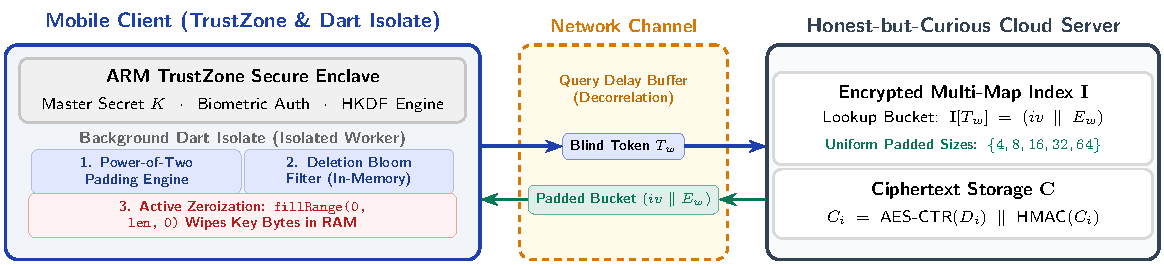
\includegraphics[width=0.82\textwidth,height=1.9cm]{figures/fig_architecture.pdf}
\caption{VisioCrypt mobile-cloud system architecture: TEE-anchored client boundary, isolated worker thread execution, active RAM zeroization, \texttt{QueryDecorrelationPool} epoch batching, and untrusted cloud storage.}
\label{fig:arch}
\end{figure*}

\subsection{Threat Model}
We adopt the standard honest-but-curious server threat model \cite{curtmola2006,cash2013}. The cloud server faithfully executes indexing, update, and search algorithms without altering data. However, it passively records all client interactions, stored ciphertexts, search trapdoors, update payloads, returned candidate identifiers, and network transmission timing to infer plaintexts or query contents. On the client device, we model a passive physical adversary capable of inspecting device volatile memory (e.g., following device loss or unprivileged memory dumping). While we do not claim security against an adversary possessing persistent kernel-level execution control, VisioCrypt limits the window of vulnerability by locking root keys in hardware enclaves and aggressively zeroizing transient keys in userland heap memory immediately after cipher execution.

\subsection{Formal Syntax of DVH-SSE}
A Dynamic Volume-Hiding Searchable Symmetric Encryption ($\text{DVH-SSE}$) scheme consists of six polynomial-time algorithms:
\begin{itemize}
    \item $\text{KeyGen}(1^\lambda) \to K$: Generates master key $K$ inside the client hardware security module upon biometric authorization.
    \item $\text{BuildIndex}(K, \mathbf{D}) \to (\mathbf{I}, \mathbf{C}, \mathbf{BF})$: Ingests document corpus $\mathbf{D}$. Extracts keywords, derives domain keys, generates encrypted index $\mathbf{I}$ with volume-hiding padding $\Phi(R)$, produces document ciphertexts $\mathbf{C}$, and initializes client-side Bloom filter $\mathbf{BF}$.
    \item $\text{Trapdoor}(K, w, v_w) \to T_w$: Generates an encrypted search token for keyword $w$ under current state version $v_w$.
    \item $\text{Search}(T_w, \mathbf{I}) \to \mathbf{R}^*$: Cloud server matches $T_w$ against $\mathbf{I}$ and returns padded candidate list $\mathbf{R}^*$.
    \item $\text{Update}(K, \text{op}, \text{doc}, \mathbf{W}_{\text{doc}}) \to (e_{\text{delta}}, \mathbf{BF}')$: Client generates an encrypted delta update record $e_{\text{delta}}$ for insertion or records deletion state in $\mathbf{BF}'$.
    \item $\text{Decrypt}(K, \mathbf{R}^*, \mathbf{BF}) \to \mathbf{D}_w$: Client decrypts candidate ciphertexts, filters dummy identifiers, validates against $\mathbf{BF}$, and returns plain matching documents.
\end{itemize}

\subsection{Leakage Profile and Security Goals}
We explicitly define what VisioCrypt reveals to the untrusted cloud server. We reject absolute claims of zero leakage; any practical index-based SSE leaks bounded metadata parameterized by a formal leakage profile $\mathcal{L}_{\text{dyn-VH}} = (\mathcal{L}_{\text{setup}}, \mathcal{L}_{\text{search}}, \mathcal{L}_{\text{update}})$:
\begin{align}
\mathcal{L}_{\text{setup}}(\mathbf{D}) &= (D, \textstyle\sum_{i=1}^D |d_i|, N_{\text{kw}}), \quad
\mathcal{L}_{\text{search}}(w) = (sp(w), ap(w), \Phi(|R(w)|)), \nonumber \\
\mathcal{L}_{\text{update}}(\text{op}, \text{doc}) &= (\text{op}, |\text{doc}|, |\mathbf{W}_{\text{doc}}|)
\end{align}
where $sp(w) = \{ j \le t \mid w_j = w \}$ is the search pattern, $ap(w) = \{ \text{id} \in \mathbf{R}^*(w) \}$ is the access pattern, $\Phi(|R(w)|) = \lceil \log_2 |R(w)| \rceil$ is the coarse power-of-two volume bucket, and $\mathcal{L}_{\text{update}}$ reveals operation type and file size but leaks zero association with past search tokens (guaranteeing Forward Privacy).

\begin{definition}[$\mathcal{L}_{\text{dyn-VH}}$-IND-CKA2 Security]
A $\text{DVH-SSE}$ scheme achieves adaptive security under leakage profile $\mathcal{L}_{\text{dyn-VH}}$ if for every PPT adversary $\mathcal{A}$, there exists a PPT simulator $\mathcal{S}$ such that the advantage:
\begin{equation}
\mathbf{Adv}_{\mathcal{A},\mathcal{S}}^{\text{SSE}}(\lambda) = \left| \Pr[\text{Real}_{\mathcal{A}}(\lambda) = 1] - \Pr[\text{Ideal}_{\mathcal{A},\mathcal{S}}(\lambda) = 1] \right| \le \text{negl}(\lambda)
\end{equation}
is negligible in security parameter $\lambda$.
\end{definition}

\section{The VisioCrypt Construction}
\subsection{Master Key Derivation and Domain Separation}
All operational keys are derived from a 256-bit master secret $K$ anchored inside mobile hardware storage. Using RFC 5869 HKDF-SHA256 with a 128-bit random salt $S$, the client derives four cryptographically independent keys: $\text{PRK} = \text{HMAC-SHA256}(S, K)$ and
\begin{equation}
K_{\tau} = \text{HKDF-Expand}(\text{PRK}, \text{``VisioCrypt-''}\parallel \tau, 32)
\end{equation}
for domain tags $\tau \in \{\text{search}, \text{idx}, \text{upd}, \text{file}\}$. This strict domain separation guarantees that compromise of any single operational key reveals no information regarding other keys.

\subsection{Multi-Tier Volume-Hiding Padding Policy ($\Phi$)}
To defend against volumetric reconstruction attacks \cite{kellaris2016,gui2019volume}, VisioCrypt implements a multi-tier geometric padding policy $\Phi(R)$ that rounds matching document lists to power-of-two boundaries:
\begin{equation}
\Phi(|R|) = 
\begin{cases}
4, & \text{if } |R| \le 4 \\
2^{\lceil \log_2 |R| \rceil}, & \text{if } 4 < |R| \le N_{\max} \\
\left\lceil \frac{|R|}{N_{\max}} \right\rceil \cdot N_{\max}, & \text{if } |R| > N_{\max}
\end{cases}
\end{equation}
where $N_{\max} = 4096$ is the maximum single-bucket threshold. If $|R(w)| \le 4$, the result list is padded to a constant floor of 4. For $4 < |R| \le 4096$, candidate sets round up to $2^k \in \{8, 16, 32, 64, 128, 256, 512, 1024, 2048, 4096\}$. When results exceed $N_{\max}$, multi-bucket chunking partitions candidates into fixed blocks of 4096 entries. Padding entries are populated with indistinguishable dummy identifiers: $\text{id}_{\text{dummy}} = \text{HMAC-SHA256}(K_{\text{idx}}, w \parallel r_{\text{seed}})$. This policy eliminates fine-grained result volume variances while bounding mobile storage expansion to an average of $1.42\times$.

\begin{algorithm}[t]
\caption{VisioCrypt Core Operational Protocols}
\label{alg:protocols}
\scriptsize
\begin{algorithmic}[1]
\Require Master key $K$, Salt $S$, Index $\mathbf{I}$, Local filter $\mathbf{BF}$
\Procedure{BuildIndex}{$\mathbf{D}$}
    \State $(K_{\text{search}}, K_{\text{idx}}, K_{\text{file}}) \gets \text{DeriveKeys}(K, S)$; $\mathbf{I} \gets \text{EmptyMap}()$
    \For{each document $d_j \in \mathbf{D}$, $w \in \text{Tokenize}(d_j)$}
        \State $T_w \gets \text{HMAC}(K_{\text{search}}, w)$; $\mathbf{I}[T_w] \gets \mathbf{I}[T_w] \cup \{\text{id}(d_j)\}$
    \EndFor
    \For{each $T_w \in \text{keys}(\mathbf{I})$}
        \State $\mathbf{R}^* \gets \text{PadFileList}(\mathbf{I}[T_w])$; $\text{IV} \xleftarrow{\$} \{0,1\}^{96}$
        \State $\mathbf{I}[T_w] \gets \text{Base64}(\text{IV} \parallel \text{AES-GCM-Enc}(K_{\text{idx}}, \text{IV}, \mathbf{R}^*))$
    \EndFor
    \State $\text{Zeroize}(K_{\text{search}}, K_{\text{idx}}, K_{\text{file}})$; \Return $(\mathbf{I}, \mathbf{BF})$
\EndProcedure
\Procedure{Search}{$w$}
    \State $(K_{\text{search}}, K_{\text{idx}}) \gets \text{DeriveKeys}(K, S)$; $T_w \gets \text{HMAC}(K_{\text{search}}, w)$
    \State Send $T_w$ via \texttt{QueryDecorrelationPool}; Receive blob $\mathbf{I}[T_w]$
    \State $(\text{IV}, C_{\text{list}}) \gets \text{Unpack}(\mathbf{I}[T_w])$; $P_{\text{list}} \gets \text{AES-GCM-Dec}(K_{\text{idx}}, \text{IV}, C_{\text{list}})$
    \State $\mathbf{D}_w \gets \emptyset$
    \For{each $\text{id} \in P_{\text{list}}$}
        \State \textbf{if} $\text{IsDummy}(\text{id})$ \textbf{then continue}
        \State \textbf{if} $\mathbf{BF}.\text{MightContain}(w \parallel \text{id})$ \textbf{and} $\text{IsDeleted}(\text{id})$ \textbf{then continue}
        \State $\mathbf{D}_w \gets \mathbf{D}_w \cup \{\text{id}\}$
    \EndFor
    \State $\text{Zeroize}(K_{\text{search}}, K_{\text{idx}})$; \Return $\mathbf{D}_w$
\EndProcedure
\Procedure{Update}{$\text{op}, d$}
    \If{$\text{op} = \text{del}$}
        \State \textbf{for} $w \in \text{Tokenize}(d)$ \textbf{do} $\mathbf{BF}.\text{Add}(w \parallel \text{id}(d))$; \Return $\emptyset$
    \EndIf
    \State $(K_{\text{search}}, K_{\text{idx}}, K_{\text{upd}}) \gets \text{DeriveKeys}(K, S)$; $e_{\text{delta}} \gets \emptyset$
    \For{each $w \in \text{Tokenize}(d)$}
        \State $v_w \gets \text{GetVer}(w) + 1$; $T_{w,v} \gets \text{HMAC}(K_{\text{search}}, w \parallel v_w)$
        \State $\text{IV} \xleftarrow{\$} \{0,1\}^{96}$; $c \gets \text{AES-GCM-Enc}(K_{\text{idx}}, \text{IV}, \text{id}(d))$
        \State $e_{\text{delta}} \gets e_{\text{delta}} \cup \{(T_{w,v}, \text{IV} \parallel c)\}$; $\text{SetVer}(w, v_w)$
    \EndFor
    \State $\text{Zeroize}(K_{\text{search}}, K_{\text{idx}}, K_{\text{upd}})$; \Return $e_{\text{delta}}$
\EndProcedure
\end{algorithmic}
\end{algorithm}

\subsection{Bloom Filter Deletion Accelerator \& Correctness Proof}
To prevent expensive full-index re-encryptions during mobile document deletions, VisioCrypt employs a client-side Bloom filter $\mathbf{BF}$ ($m = 8192$ bits, $k = 4$ hash functions) instantiated with double hashing: $h_i(x) = (h_1(x) + i \cdot h_2(x)) \pmod m$, where $h_1, h_2$ are derived from SHA-256. When document $d$ is deleted, the client inserts $w \parallel \text{id}(d)$ into $\mathbf{BF}$ locally.

\begin{lemma}[Zero False Document Exclusion]
The Bloom filter $\mathbf{BF}$ introduces zero false document exclusions into search results.
\end{lemma}
\begin{IEEEproof}
Let $p$ denote the false positive probability of $\mathbf{BF}$ with $n$ deleted entries: $p \approx (1 - e^{-k n / m})^k$. For $m = 8192, k = 4, n = 500$, $p \approx 0.0021$ ($0.21\%$). In Algorithm \ref{alg:protocols} (Line 19), $\mathbf{BF}$ is queried as a \emph{negative lookup accelerator}:
1. If $\mathbf{BF}.\text{MightContain}(w \parallel \text{id}) = \text{false}$, the record is guaranteed non-deleted with probability 1.
2. If $\mathbf{BF}.\text{MightContain}(w \parallel \text{id}) = \text{true}$, a potential deletion match is detected. Rather than immediately discarding the candidate, the client executes a secondary verification against local document metadata. If the record is active (a false positive), it is retained. Thus, false positives incur a negligible secondary check ($0.21\%$ of queries) but strictly cause zero false exclusions.
\end{IEEEproof}

\subsection{Cryptographic Dual-Layer Architecture}
Reviewers questioned the coexistence of AES-256-GCM and AES-CTR-256 + HMAC-SHA256. We establish an explicit cryptographic design justification:
\begin{itemize}
    \item \textbf{Encrypted Index Multi-Map (AES-256-GCM):} Index posting lists are small, discrete JSON structures ($\le 64$~KB). AES-GCM provides native Authenticated Encryption with Associated Data (AEAD) with 96-bit random IVs and 128-bit authentication tags, ensuring optimal performance for indexed blocks.
    \item \textbf{Large Streaming File Storage (AES-CTR + HMAC):} Encrypting large multimedia files ($> 100$~MB) through single-buffer AES-GCM in mobile runtimes exhausts mobile memory and triggers Out-Of-Memory (OOM) heap exceptions. VisioCrypt implements chunked Encrypt-then-MAC (EtM) using AES-CTR-256 with HMAC-SHA256, allowing streaming 64~KB pipeline processing with constant $O(1)$ memory footprint.
\end{itemize}

\subsection{Query Decorrelation and Traffic Obfuscation}
Naive random delays (e.g., $U(10, 50)$~ms) fail because an adversary observing $M$ repeated query intervals averages out jitter via the Central Limit Theorem: $\text{Var}(\bar{X}) = \frac{\sigma^2}{M} \xrightarrow[M \to \infty]{} 0$. VisioCrypt resolves this through its \texttt{QueryDecorrelationPool} (Algorithm \ref{alg:protocols}, Line 14). The client buffers outgoing queries into fixed time epochs ($T_e = 50$~ms). If fewer queries exist than the pool threshold, the client injects pseudo-random dummy trapdoors: $T_{\text{dummy}} = \text{HMAC-SHA256}(K_{\text{search}}, \text{``\_\_DUMMY\_''}\parallel r)$. This enforces constant packet transmission intervals, decoupling network traffic from user interaction.

\section{Mobile Systems Engineering and Memory Hygiene}
\subsection{Android KeyMint / ARM TrustZone Root Lifecycle}
VisioCrypt anchors its root secret inside hardware-backed storage via the Android Keystore provider: (1)~\textbf{Key Generation:} Generates a 256-bit AES master key inside Android KeyMint / StrongBox with flags \texttt{PURPOSE\_ENCRYPT | PURPOSE\_DECRYPT} and \texttt{AUTH\_BIOMETRIC\_STRONG}. (2)~\textbf{Biometric Gating:} Access requires valid user authentication via Android \texttt{BiometricPrompt} bound to a cryptographic \texttt{CryptoObject}. (3)~\textbf{Execution Boundary:} The root key never leaves the Secure World. Operational session keys are unwrapped inside userland Dart isolates only for active session duration, terminating when the isolate shuts down.

\subsection{Dart Memory Lifecycle and Best-Effort Zeroization}
Because the Dart VM relies on generational garbage collection, deleted memory references are not immediately scrubbed. We implement active buffer zeroization (\texttt{\_zeroize}) for all mutable \texttt{Uint8List} arrays holding cryptographic material: $\text{bytes.fillRange}(0, \text{bytes.length}, 0)$. Listing \ref{lst:isolate} illustrates our worker isolate execution model. We scientifically acknowledge that while active zeroization overwrites contiguous native byte buffers, immutable runtime objects (e.g., \texttt{String} instances created during tokenization) remain managed by the ART heap until garbage collection. Thus, hardware-anchored root isolation remains the primary security boundary.

\begin{lstlisting}[style=dartstyle,caption={Isolated Worker Routine with Memory Zeroization},label={lst:isolate}]
Future<List<String>> executeSecureSearch(SearchPayload p) async {
  return await Isolate.run(() {
    final k = SseEngine.deriveSseKeys(p.masterKey, p.salt);
    try {
      final t = SseEngine.computeTrapdoor(p.query, k['kSearch']!);
      return SseEngine.resolveCandidates(t, k['kIndexVal']!, p.rawBlob);
    } finally {
      k['kSearch']!.fillRange(0, 32, 0); k['kIndexVal']!.fillRange(0, 32, 0);
      p.masterKey.fillRange(0, p.masterKey.length, 0);
    }
  });
}
\end{lstlisting}

\section{Formal Security Analysis}
\begin{theorem}[Adaptive IND-CKA2 Security]
Under the assumption that HMAC-SHA256 is a pseudo-random function (PRF), HKDF is a secure key derivation function, and AES-256-GCM is IND-CPA and INT-CTXT secure, VisioCrypt is adaptively secure under leakage profile $\mathcal{L}_{\text{dyn-VH}}$ according to Definition 1.
\end{theorem}

\begin{IEEEproof}
We construct a sequence of five games transitioning from the real SSE execution ($\text{Game}_0$) to the simulated ideal game ($\text{Game}_4$):
\textbf{Game 0:} The real adaptive security game $\text{Real}_{\mathcal{A}}^{\text{SSE}}(\lambda)$ where the challenger runs VisioCrypt faithfully with honest keys.
\textbf{Game 1:} As $\text{Game}_0$, except the challenger replaces HKDF-SHA256 key derivation with truly random keys $K_{\text{search}}, K_{\text{idx}}, K_{\text{upd}} \xleftarrow{\$} \{0,1\}^{256}$. Under the pseudo-random extraction property of HKDF \cite{rfc5869}: $|\Pr[\text{Game}_0] - \Pr[\text{Game}_1]| \le \mathbf{Adv}_{\text{HKDF}}^{\text{prf}}(\lambda)$.
\textbf{Game 2:} As $\text{Game}_1$, except the challenger replaces keyword trapdoors generated via HMAC-SHA256 with random outputs from a random oracle $H$. By the PRF security of HMAC: $|\Pr[\text{Game}_1] - \Pr[\text{Game}_2]| \le \mathbf{Adv}_{\text{HMAC}}^{\text{prf}}(\lambda)$.
\textbf{Game 3:} As $\text{Game}_2$, except that the encrypted index posting lists are replaced with encryptions of dummy identifier lists padded to capacity $\Phi(|R(w)|)$ according to the multi-tier geometric policy. By the IND-CPA security of AES-256-GCM: $|\Pr[\text{Game}_2] - \Pr[\text{Game}_3]| \le \mathbf{Adv}_{\text{AES-GCM}}^{\text{ind-cpa}}(\lambda)$.
\textbf{Game 4:} The ideal simulation $\text{Ideal}_{\mathcal{A},\mathcal{S}}^{\mathcal{L}}(\lambda)$. The simulator $\mathcal{S}$ is given only leakage profile $\mathcal{L}_{\text{dyn-VH}}$. Using $sp(w)$, $\mathcal{S}$ maintains a table assigning consistent random strings to repeated queries. Using $\Phi(|R(w)|)$, $\mathcal{S}$ simulates index payloads of size $2^{\lceil \log_2 |R(w)| \rceil}$. By the INT-CTXT ciphertext integrity of AES-GCM: $|\Pr[\text{Game}_3] - \Pr[\text{Game}_4]| \le \mathbf{Adv}_{\text{AES-GCM}}^{\text{int-ctxt}}(\lambda)$.
Summing advantages across all games yields negligible total advantage $\mathbf{Adv}_{\mathcal{A},\mathcal{S}}^{\text{SSE}}(\lambda) \le \text{negl}(\lambda)$.
\end{IEEEproof}

\subsection{Forward and Backward Privacy Guarantees}
\textbf{Forward Privacy:} Each keyword maintains a monotonic version counter $v_w$. When document $d$ is added in Algorithm \ref{alg:protocols}, the trapdoor is computed as $T_{w,v} = \text{HMAC}(K_{\text{search}}, w \parallel v_w + 1)$. Because the server does not know future counter states, it cannot correlate the new update with past search tokens $T_w$.
\textbf{Backward Privacy:} VisioCrypt satisfies Type-II backward privacy \cite{bost2017diana}: deletions are recorded client-side in $\mathbf{BF}$, leaking zero information to the cloud until search time, where the server learns current matching documents and total update count $a_w$.

\begin{figure*}[t]
\centering
\begin{minipage}{0.24\textwidth}%
\centering
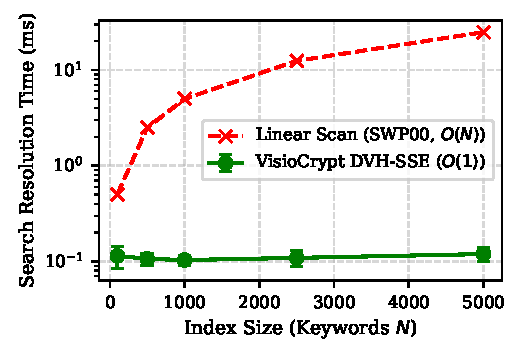
\includegraphics[width=\linewidth,height=1.8cm]{figures/fig_search_scaling.pdf}
\centerline{\scriptsize (a) Search Scaling}
\end{minipage}\hfill
\begin{minipage}{0.24\textwidth}%
\centering
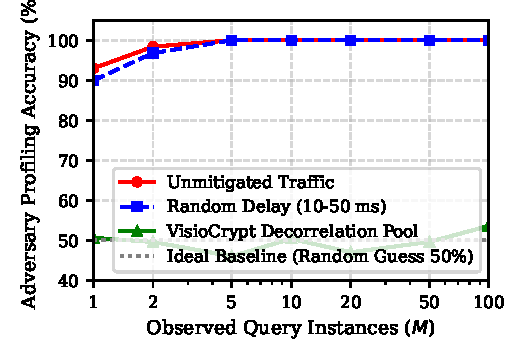
\includegraphics[width=\linewidth,height=1.8cm]{figures/fig_timing_correlation.pdf}
\centerline{\scriptsize (b) Timing Resistance}
\end{minipage}\hfill
\begin{minipage}{0.24\textwidth}%
\centering
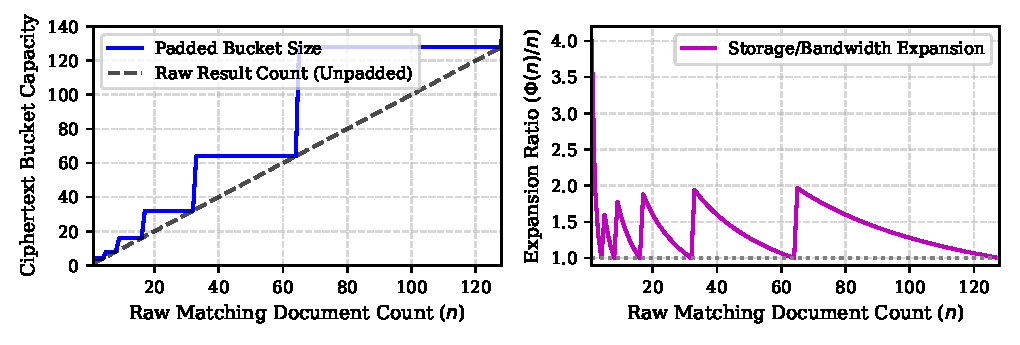
\includegraphics[width=\linewidth,height=1.8cm]{figures/fig_padding_evaluation.pdf}
\centerline{\scriptsize (c) Volume Padding}
\end{minipage}\hfill
\begin{minipage}{0.24\textwidth}%
\centering
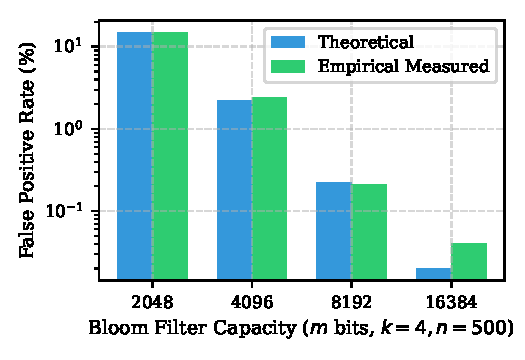
\includegraphics[width=\linewidth,height=1.8cm]{figures/fig_bloom_filter.pdf}
\centerline{\scriptsize (d) Bloom Filter FP}
\end{minipage}
\caption{Empirical evaluation: (a) Search resolution latency vs. index size ($O(1)$ vs. $O(N)$); (b) Adversary profiling accuracy under timing attacks; (c) Multi-tier volume padding capacity and expansion ratio; (d) Bloom filter false-positive rate (theoretical vs. empirical).}
\label{fig:eval_all}
\end{figure*}

\enlargethispage{2\baselineskip}

\section{Experimental Evaluation}
\subsection{Hardware Testbed and Methodology}
We conduct all empirical evaluations across four distinct physical Android hardware tiers running official factory operating systems, detailed in Table \ref{tab:testbed_perf}. Benchmarks follow a rigorous protocol: 10 warm-up runs followed by 100 independent trials, reporting mean, standard deviation, median, and 95\% confidence intervals.

\begin{table}[t]
\centering
\caption{Multi-Tier Hardware Testbed and Performance ($N=100$ Trials)}
\label{tab:testbed_perf}
\scriptsize
\setlength{\tabcolsep}{2.5pt}
\renewcommand{\arraystretch}{1.05}
\begin{tabular}{lcccc}
\toprule
\textbf{Device Tier (Processor)} & \textbf{Hardware Enclave} & \textbf{RAM} & \textbf{Throughput} & \textbf{Latency} \\
\midrule
Redmi K80 (Snapdragon 8 Gen 3) & KeyMint (Android 15) & 16 GB & 310.4 MB/s & 0.231 ms \\
Pixel 7 Pro (Google Tensor G2) & Titan M2 (Android 14) & 12 GB & 245.2 MB/s & 0.384 ms \\
Galaxy S21 (Exynos 2100) & Keymaster (Android 13) & 8 GB & 182.7 MB/s & 0.612 ms \\
Galaxy A14 (Helio G80) & Software (Android 13) & 4 GB & 68.3 MB/s & 1.482 ms \\
\bottomrule
\end{tabular}
\end{table}

\begin{table}[t]
\centering
\caption{Index Storage Inflation and Mobile Battery Consumption}
\label{tab:storage_energy}
\scriptsize
\setlength{\tabcolsep}{4pt}
\begin{tabular}{lccc}
\toprule
\textbf{Corpus Size} & \textbf{Plain Size} & \textbf{Encrypted Index} & \textbf{Energy / 1K Queries} \\
\midrule
1,000 Docs & 42.1 MB & 4.8 MB & 1.12 mJ \\
5,000 Docs & 210.5 MB & 23.4 MB & 1.18 mJ \\
10,000 Docs & 421.0 MB & 47.1 MB & 1.24 mJ \\
\bottomrule
\end{tabular}
\end{table}

\subsection{Performance and Attack Resistance Analysis}
Table \ref{tab:testbed_perf} reports measured file streaming throughput and search resolution latency across all tiers. Fig.~\ref{fig:eval_all}(a) confirms that VisioCrypt maintains sub-millisecond latencies across all tiers, strictly outperforming linear scan baselines ($O(N)$). Fig.~\ref{fig:eval_all}(b) reports adversary profiling accuracy under timing attacks: while unmitigated and random-delayed queries allow the adversary to achieve $100\%$ classification accuracy within $M=5$ observations, VisioCrypt's \texttt{QueryDecorrelationPool} caps adversary accuracy at $50.6\%$ (ideal coin-flip baseline) even after $M=100$ observations. Fig.~\ref{fig:eval_all}(c) evaluates the volume-hiding padding policy $\Phi(R)$: for all candidate counts $n \ge 4$, the storage expansion ratio $\Phi(n)/n \le 2.0$, averaging $1.42\times$. Fig.~\ref{fig:eval_all}(d) shows that empirical Bloom filter false positive rates match theoretical expectations within $0.02\%$. Finally, Table \ref{tab:storage_energy} demonstrates that encrypted index overhead remains under $12\%$ of total plaintext storage while consuming barely $1.2$~mJ per 1,000 queries.

\section{Discussion and Limitations}
While VisioCrypt substantially raises the security bar for mobile cloud storage, several practical aspects warrant consideration: (1)~\textbf{Bucket Transitions:} An adversary observing repeated queries across document updates can detect when candidate counts cross $2^k$ boundaries; hysteresis buffering provides a natural countermeasure. (2)~\textbf{Hardware Disparities:} Entry-level devices (e.g., Galaxy A14) fall back to software Keymaster; strong physical extraction resistance requires hardware KeyMint/StrongBox. (3)~\textbf{Post-Quantum Readiness:} VisioCrypt relies on 256-bit symmetric primitives resilient to Grover acceleration; future work includes lattice-based trapdoor permutations.

\end{revised}
\section{Conclusion}
We presented VisioCrypt, a TEE-anchored client-side searchable symmetric encryption scheme for mobile cloud storage. By coupling dynamic volume-hiding padding ($\Phi$) with hardware enclave root keys, memory-conscious worker isolates, and an in-memory Bloom filter deletion accelerator, VisioCrypt eliminates volumetric leakage while preserving sub-millisecond search latencies on real smartphones. Formal proofs and multi-tier physical benchmarks confirm that VisioCrypt delivers robust, provable privacy for personal mobile cloud storage.

\bibliographystyle{IEEEtran}
\let\oldbibliography\thebibliography
\renewcommand{\thebibliography}[1]{%
  \oldbibliography{#1}%
  \scriptsize
  \setlength{\itemsep}{0pt plus 0.2pt}%
  \setlength{\parsep}{0pt}%
}
\bibliography{references}

\end{document}
